% Template for a Computer Science Tripos Part II project dissertation
\documentclass[12pt,a4paper,twoside,openright]{report}
\usepackage[pdfborder={0 0 0}]{hyperref}    % turns references into hyperlinks
\usepackage[left=25mm, right=25mm, bottom=25mm, top=20mm]{geometry}  % adjusts page layout
\usepackage{graphicx}  % allows inclusion of PDF, PNG and JPG images
\usepackage{verbatim}
\usepackage{amsfonts}
\usepackage{placeins}
\usepackage{amsthm}
\usepackage{amsmath}
\usepackage{tabu}
\usepackage{docmute}   % only needed to allow inclusion of proposal.tex
\usepackage[utf8]{inputenc}
\usepackage{mathtools}
\usepackage{changepage}
\usepackage{url}
\usepackage{blindtext}
\usepackage{tabularx,booktabs}
\usepackage{dirtree}
\usepackage{cite}
\usepackage{float} % Prevent Latex from repositioning tables
\usepackage{graphicx}

%--- Remove hbox warning
\hfuzz=5000.002pt 
%----------------------------------------------------------------------------------------

% Formatting Commands
\newcommand{\keyword}[1]{\textbf{#1}}
\newcommand{\tabhead}[1]{\textbf{#1}}
\newcommand{\code}[1]{\texttt{#1}}
\newcommand{\file}[1]{\texttt{\bfseries#1}}
\newcommand{\option}[1]{\texttt{\itshape#1}}

%----------------------------------------------------------------------------------------
%% *****************************************************************
\newlength{\upBranch} % shift up the text  lines <<<<
\setlength{\upBranch}{0.7ex} % 

\newlength{\tolineSpace} % blank space bellow text  lines  <<<
\setlength{\tolineSpace}{1mm}% 

\usepackage{xpatch} % needed <<<<<<<<
\makeatletter

\xpatchcmd{\dirtree} % root
{\vbox{\@nameuse{DT@body@1}}}
{\raisebox{-\tolineSpace}{\vbox{\@nameuse{DT@body@1}}}}
{}{}    

\xpatchcmd{\dirtree} % below space
{\advance\dimen\z@ by-\@nameuse{DT@lastlevel@\the\DT@countiv}\relax}
{\advance\dimen\z@ by-\tolineSpace \advance\dimen\z@ by-\@nameuse{DT@lastlevel@\the\DT@countiv}\relax}
{}{}
    
\xpatchcmd{\dirtree}% shift up the text  lines
{\kern\DT@sep\box\z@\endgraf}
{\kern\DT@sep\raisebox{-\upBranch}{\box\z@}\endgraf}
{}{}    

\makeatother
%% *****************************************************************


%-----
% Language setting
\usepackage[english]{babel}
%\raggedbottom                           % try to avoid widows and orphans
\sloppy
\clubpenalty1000%
\widowpenalty1000%

\renewcommand{\baselinestretch}{1.1}    % adjust line spacing to make
                                        % more readable


\theoremstyle{definition}
\newtheorem{definition}{Definition}[section]
\graphicspath { {figs/}}

\begin{document}

% Change these

\newcommand{\mcandidate}{2200D}
\newcommand{\mfullname}{Judah Daniels}
\newcommand{\mcollege}{Clare College}
\newcommand{\mtitle}{Inferring Harmony from Free Polyphony}
\newcommand{\ntitle}{Inferring Harmony from Free Polyphony}
\newcommand{\mexamination}{Computer Science Tripos -- Part II}
\newcommand{\mdate}{July, 2023}
\newcommand{\moriginator}{Christoph Finkensiep}
\newcommand{\msupervisor}{Dr Peter Harrison}
\newcommand{\mwordcount}{5434}
\newcommand{\mlinecount}{2272}
% Consent to the dissertation made available to University members
\newcommand{\mconsent}{I am content for my dissertation to be made available to the students and staff of the University.}
% For the Declaration of originality
\newcommand{\msignature}{Judah Daniels}


\bibliographystyle{acm}

%%%%%%%%%%%%%%%%%%%%%%%%%%%%%%%%%%%%%%%%%%%%%%%%%%%%%%%%%%%%%%%%%%%%%%%%
% Title
%%%%%%%%%%%%%%%%%%%%%%%%%%%%%%%%%%%%%%%%%%%%%%%%%%%%%%%%%%%%%%%%%%%%%%%%

\thispagestyle{empty}

\rightline{\LARGE \textbf{\mfullname}}

\vspace*{60mm}
\begin{center}
\Huge
\textbf{\mtitle} \\[5mm]
\mexamination \\[5mm]
\mcollege \\[5mm]
\mdate  % today's date
\end{center}

%%%%%%%%%%%%%%%%%%%%%%%%%%%%%%%%%%%%%%%%%%%%%%%%%%%%%%%%%%%%%%%%%%%%%%%%%%%%%%
% Proforma, table of contents and list of figures
%%%%%%%%%%%%%%%%%%%%%%%%%%%%%%%%%%%%%%%%%%%%%%%%%%%%%%%%%%%%%%%%%%%%%%%%%%%%%%

\pagestyle{plain}

\newpage
\newpage
\section*{Declaration of originality}

I, \mfullname{} of \mcollege, being a candidate for Part II of the Computer Science Tripos, hereby declare that this dissertation and the work described in it are my own work, unaided except as may be specified below, and that the dissertation does not contain material that has already been used to any substantial extent for a comparable purpose. \mconsent

\bigskip
\leftline{Signed \msignature}
\bigskip
\leftline{Date \today}

\chapter*{Proforma}


{\large
\begin{tabular}{ll}
Candidate Number:   & \bf \mcandidate                   \\
Project Title:      & \bf \mtitle                       \\
Examination:        & \bf \mexamination, \mdate         \\
Word Count:         & \bf \mwordcount\footnotemark[1]   \\
Code Line Count:    & \bf \mlinecount                   \\
Project Originator: & \bf \moriginator                  \\
Supervisor:         & \bf \msupervisor                  \\ 
\end{tabular}
}

\footnotetext[1]{This word count was computed
by \texttt{detex diss.tex | tr -cd '0-9A-Za-z $\tt\backslash$n' | wc -w}
}
\stepcounter{footnote}


\section*{Original Aims of the Project}
% At most 100 words



\section*{Work Completed}
% At most 100 words

All that has been completed appears in this dissertation.

\section*{Special Difficulties}
% At most 100 words

None

\newpage

\tableofcontents

\listoffigures

\newpage
\section*{Acknowledgements}



%%%%%%%%%%%%%%%%%%%%%%%%%%%%%%%%%%%%%%%%%%%%%%%%%%%%%%%%%%%%%%%%%%%%%%%
% now for the chapters

\pagestyle{headings}

\chapter{Introduction}
\textit{This dissertation explores efficient search strategies for parsing a symbolic music data using a musical grammar. We present ... which extends a recent model, addressing problems of intractability by using Heuristic search methods. We will see that that my novel heuristic search algorithm achieves .... }

\section{Motivation}

A piece of music can be described using a sequence of chords, representing a higher level harmonic structure of a piece. There is a small, finite set of chord types, but each chord can be realised on the musical surface in a practically infinite number of ways. Given a score, we wish to infer the underlying chord types. This is often a time consuming and cognitively demanding expert task \cite{masadaChordRecognitionSymbolic2018}, hence its utility.

\par
The paper \textit{Modeling and Inferring Proto-voice Structure in Free Polyphony} describes a generative model that encodes the recursive and hierarchical dependencies between notes, giving rise to a grammar-like hierarchical system \cite{finkensiepMODELINGINFERRINGPROTOVOICE2021}. This proto-voice model can be used to reduce a piece into a hierarchical structure which encodes an understanding of the tonal/harmonic relations.
\par
Finkensiep suggests in his thesis that the proto-voice model may be an effective way to infer higher level latent entities, such as harmonies or voice leading schemata. Thus in this project I will ask the question: is this parsing model an effective way to annotate harmonies? By ‘effective’ we are referring to two things:
\begin{itemize}
  \item Accuracy: can the model successfully emulate how experts annotate harmonic progressions in musical passages? 
  \item Practicality: can the model be used to do this within a reasonable time frame?
\end{itemize}

While the original model could in theory be used to generate harmonic annotations, its exhaustive search strategy would be prohibitively time-consuming in practice for any but the shortest musical extracts; one half measure can have over 100,000 valid derivations \cite{finkensiepStructureFreePolyphony2023}. My approach will be to explore the use of heuristic search algorithms to solve this problem.

\section{Related Work}
First grammar/rule-based systems \cite{maxwellExpertSystemHarmonizing1992} \cite{winogradLinguisticsComputerAnalysis1968}, optimisation algorithms \cite{pardoAlgorithmsChordalAnalysis2002} and supervised learning approaches making use of large datasets \cite{niEndtoendMachineLearning2011} \cite{mcleodModularSystemHarmonic2021} \cite{masadaChordRecognitionSymbolic2018}.
\par
Distinction to be drawn between approaches that take segmented or non-segmented pieces. Some models make use of a joint segmentation and labelling approach \cite{masadaChordRecognitionSymbolic2018}... 

\par
More general heuristic search techniques for huge search spaces.

%%%%%%%%%%%%%%%%%%%%%%%%%%%%%%%%%%%%%%%%%%%%%%%%%%%%%%%%%%%%%%%%%%%%%
% Preparation
%%%%%%%%%%%%%%%%%%%%%%%%%%%%%%%%%%%%%%%%%%%%%%%%%%%%%%%%%%%%%%%%%%%%%

\chapter{Preparation}
\textit{In this chapter, I present the work which was undertaken before the code was written. After a brief description of my starting point, I provide an exposition of the Proto-voice Model which forms the foundation of this project. Subsequently, I discuss probabilistic programming and Bayesian inference, including a probabilistic model of harmony. Finally, I describe the software engineering techniques and principles used throughout the project. }

\section{Background Material}

\subsection{Proto-voice Model}
TODO: Brief description of what notes are, what is a piece of music, introduce relevant musical terminology (Score, note, protovoice, repetition, neighbor/ ornament(choose one?)). Conflict of meaning with root-note (generative operation) and root note (musical terminology). What are the main assumptions/ information we need to know in order to understand the proto-voice model?

\par
TODO: Motivation of the model as a generative model on the note level, describing the piece as a DAG (Directed Acyclic Graph). What is a proto-voice exactly? 
\par 

The proto-voice model is characterised by 3 primitive generative operations on notes.

\begin{itemize}
  % \setlength\itemsep{1em}
 \item Repetitions 
  \item Neighbor notes 
  \item Passing notes
\end{itemize}

Operations with two notes are represented by edge replacement. 
\[p_1 \to p_2 ~~~\implies~~ p_1 \to c \to p_2 \label{edge replacement}\]

\subsubsection{Proto-voice Operations}

To model simulataneity of notes we introduce slices, which are multisets of pitches, representing segments of a piece where a group of notes are heard. 
\par 
Diagram showing a slice + a diagram showing a higher level slices, grouping an arpegiation.
\par 
A slice $m$ is defined as a multiset of pitches.
\par 
A transition $t = (s_l, e, s_r)$  relates two slices with a configuration of edges $e=(e_{reg}, e_{pass})$, a set of regular edges (repetition or neighbor), and a set of passing edges.
\par
Outer operations (Diagram of all three operations): 
\par
Split: \[t \to t'_l s' t'_r\]
Spread: \[t_l~s~t_r \to t'_l~s'_l~t'_m~s'_r~t'_r\]
Freeze: \[t \to t \]

\subsubsection{Proto-voice harmony}
How do we get from a proto-voice (partial)derivation to a harmonic inference?
\par
Explain what harmony is, and how the proto-voice model allows us to capture harmony. Elaboration of the introduction.
\par
What assumptions are needed for a protovoice derivation to be able to describe harmonic entities? These shape heuristic design.
\par


\subsection{Probabilistic Programming}
Provide an explanation of all the concepts I learned and used in this project. 
Techniques such as marginalisation, joint distributions, bayes rule etc. 
Probabilistic programming is the combination model definitions and statistical inference algorithms for computing the conditional distribution of inputs (chords) that could have given rise to the observed output (score). We are making the assumption that the score is a realisation of the latent harmonic entities. 

Dirchelet distributions
Beta distribution  
Multinomiall distribution 
Normal Distribution 

\par 
Inference as model $\to$ data $\to$ prob distribution $\to$ chord guess

\subsection{Probabilistic Model of Harmony}

Outline of the probabilistic model of harmony, describing the parts that are relevant for harmonic annotations. This section allows the reader to understand the evaluation and heuristic modules.

\par
Describe how the parameters were attained
\par
Then describe how to go from the parameters to chord, chordtone and ornamentation distributions
\par

Parameters:
\par
pHarmonies: $\mathbb{N}^{n_c}$\\
pChordtones: $\mathbb{N}^{n_c}$\\
pOrnaments: $\mathbb{N}^{n_c}$
\par
Chordtypes, $C = \{\text{M,~m, Mm7, om, o7, mm7, \%7, MM7, +, Ger, It, Fr, mM7, +7}\}$

\[\vec{\chi}' \sim \text{Dirchlet} (\text{pHarmonies}, n_c) \]

\[\vec{\chi} = \mathbb{E} (\vec{X}_i) = \frac{\alpha_i}{\sum\limits_j \alpha_j} \]

Chord: \[c \sim \text{Categorical}(\vec{\chi})\]

Single chordtone distribution. We want to find $P(p|c, ct)$ probability of the pitch given the chord, and that the note is a chordtone:
\[\vec{\phi}_{ct}' \sim \text{Dirchlet}(pChordtones, n_p) \implies \vec{\phi}\]

For each of these parameters we use the MLE to get our probability distribution. 
\[\vec{\phi}_{ct} = \text{MLE} (\vec{\phi}_{ct}')\]
\[\vec{\phi}_{or} = \text{MLE} (\vec{\phi}_{or}')\]
\[\vec{\chi}= \text{MLE} (\vec{\chi}') \]
Then for each chord tone,
\[p_{ct} \sim \text{Categorical}(\vec{\phi}_{ct})\]
\[p_{or} \sim \text{Categorical}(\vec{\phi}_{or})\]
We get the distribution of likelihoods for each pitch.






\subsection{Heuristic Search Algorithms}

Provide an outline of the heuristic search paradigm with a formalisation.
\par
Provide a brief overview of different techniques that are used to prune the search space that might be relevant.

\section{Starting Point}

\subsection{Relevant courses and experience}

\paragraph{Haskell}{I was introduced to Haskell during an internship during the summer before starting this project (July to August 2022). This project is an excuse to learn the language.}
\paragraph{Python}{I have experience coding in Python.}

\paragraph{IB}{ Formal Models of Language, Artificial Intelligence.}

\subsection{Existing codebase}
NOTE: I need to restructure the codebase to reflect the different modules more clearly. This will help with the flow to the dissertation.

The following describes the protovoices-haskell repository, and where my code contribution will lie:
\par
\medskip
\dirtree{%
.1 protovoices-haskell.
.2 app.
.3 MainExamples.hs.
.3 MainISMIR.hs.
% .3 MainLearning.hs.
% .3 MainHeuristicSearch.hs <- My code.
.3 ....
.2 src.
.3 \textbf{Heuristics} <- My code.  
% .4 …  <- My code.
.3 ....
.2 test.
% .2 testdata.
.2 ....
}

\section{Requirements Analysis}

Table of main components with a dependency and risk analysis 

\begin{table}[ht]
  \caption{Overview of main deliverables along with a risk analysis}
  \label{requirements}
  \begin{tabularx}{\textwidth}{cXcc}
    ID & Delieverable & Priority & Risk \\
    \toprule
    \texttt{core1} & Evaluation Module & High & Low \\
    \texttt{core2} & End to End Pipeline  & High & Medium \\
    \texttt{core3} & Parser  & High & Medium \\
    \texttt{base1} & Random Choice search & High & Low \\
    \texttt{base2} & Random Sample & High & Low \\
    \texttt{ext1} & Heuristic Search 1 & Medium & High \\
    \texttt{ext2} & Heuristic Search 2 & Medium & High \\
  \end{tabularx}
\end{table}
\par
Short description of where the risk lies. 
\par
Pertt chart showing the dependencies between different modules


\section{Software Engineering Techniques}
Justified and documented selection of suitable tools; good engineering approach.


\subsection{Development model}

Usig the dependency and risk analysis above, I created this gantt chart, and totally stuck to it(100\% didn't wait until now to get the end-to-end pipeline fully running, and spend most of the time in an extension rabbit hole.. We live and we learn).

Include Gantt chart.

\subsection{Languages, libraries and tools}
The chapter will also cite any new programming languages and systems which had to be learnt 

\begin{table}
  {
  \small
  \caption{Languages, libraries and tools}
  \label{Languages}
  \begin{center}
    \begin{tabularx}{.9\textwidth}{cXc}
      Tool & Purpose & License \\
      \toprule
      Haskell & Main language & ... \\
      \midrule
      GHC & Compiling and profiling to inspect time performance and memory usage  & GPL-3.0+ \\
      \midrule
      Haskell-Musicology & ... & ... \\
      \midrule
      Dimcat & ... & ... \\
      \midrule
      Python & ... & ... \\
      \midrule
      Numpy & ... & ... \\
      \midrule
      Pandas & ... & ... \\
      \midrule
      MS3 & ... & ... \\
      \midrule
      Musescore 3 & ... & ... \\
      \midrule
      Protovoice Annotation Tool & ... & ... \\
      \midrule
      Git & Version Control, Continuous Integration & ... \\
      \bottomrule
    \end{tabularx}
  \end{center}
  }
\end{table}

%%%%%%%%%%%%%%%%%%%%%%%%%%%%%%%%%%%%%%%%%%%%%%%%%%%%%%%%%%%%%%%%%%%%%
% Implementation
%%%%%%%%%%%%%%%%%%%%%%%%%%%%%%%%%%%%%%%%%%%%%%%%%%%%%%%%%%%%%%%%%%%%%

\chapter{Implementation}

\section{Repository Overview:}

Insert block diagram of components here.

\vspace{50\baselineskip}

\DTsetlength{0em}{1.3em}{0em}{0.7pt}{3pt}       
\setlength{\DTbaselineskip}{15pt}  %minimum size for \normalsize
\renewcommand{\DTstyle}{\ttfamily}

\begin{table}[!t]
  % \centering
  \caption{Repository Overview}
  \vspace{\baselineskip}
  \label{jeff}
  \begin{tabularx}{\textwidth}{l X c}
    File/Folder & Description & LOC \\
    \toprule
    \toprule
  \begin{minipage}[t]{5.3cm}
    \dirtree{%
    .1 protovoices-haskell/.
    .2 src/.
    .3 HeuristicParser.hs,~HeuristicSearch.hs \vspace{\DTbaselineskip}.
    .3 RandomChoiceSearch.hs,~RandomSampleParser.hs\vspace{2\DTbaselineskip}.
    .3 Heuristics.hs,~PBHModel.hs \vspace{2\DTbaselineskip}.
    .3 FileHandling.hs\vspace{2\DTbaselineskip}.
    .3 \dots \vspace{\DTbaselineskip}.
    .2 app/.
    .3 MainFullParse.hs\vspace{\DTbaselineskip}. 
    .2 harmonic-inference \vspace{\DTbaselineskip}.
    .2 experiments/.
    .3 preprocess.ipynb.
    .3 dcml\_params.json.
    .3 inputs/ \vspace{\DTbaselineskip}.
    .2 test/ \vspace{\DTbaselineskip}.
    }
  \end{minipage} &
  \begin{minipage}[t]{8cm}
Root directory
\vspace{2\baselineskip}\\
Core Implementation (Section x)
\vspace{2\baselineskip}\\
Baseline Implemetation (Section x)
\vspace{2\DTbaselineskip}\\
Extension Implementation (Section x) 
\vspace{2\DTbaselineskip}\\
Utilities
\vspace{5\DTbaselineskip}\\
Entry Point
\vspace{8.2\DTbaselineskip}\\
Unit Tests (Section x)

  \end{minipage} & 
  \begin{minipage}[t]{0.5cm}
    2272
    \vspace{0.1\DTbaselineskip}\\
    470\\
    \vspace{\DTbaselineskip}
    121\\
    \vspace{\DTbaselineskip}
    383\\
    \vspace{1.8\DTbaselineskip}
    188\\
    \vspace{3.7\DTbaselineskip}
    431\\
    \vspace{3\DTbaselineskip}
    115\\
    \vspace{2.5\DTbaselineskip}
    611\\
  \end{minipage}
\end{tabularx}
\end{table}

The following describes an overview of the project repository:

\section{Core Implementation}

\subsection{Heuristic Parser}
This is not a descriptive name. Think of a new name to describe the implementation of the search space of partial reductions. We use the outer representation of structure and outer operations. This is an abstraction.

\subsubsection{Parsing Operations}
Piece represented by an alternating list of slices and transitions, this is called a path. Define path formally. inductive definitions. dont need the Nothing: just Path trans slice. Transition can be frozen or unfrozen, and boundary or non boundary. Boundary is represented by vertical line, frozen is represented by two lines.

\begin{figure}[ht]
  \centering
  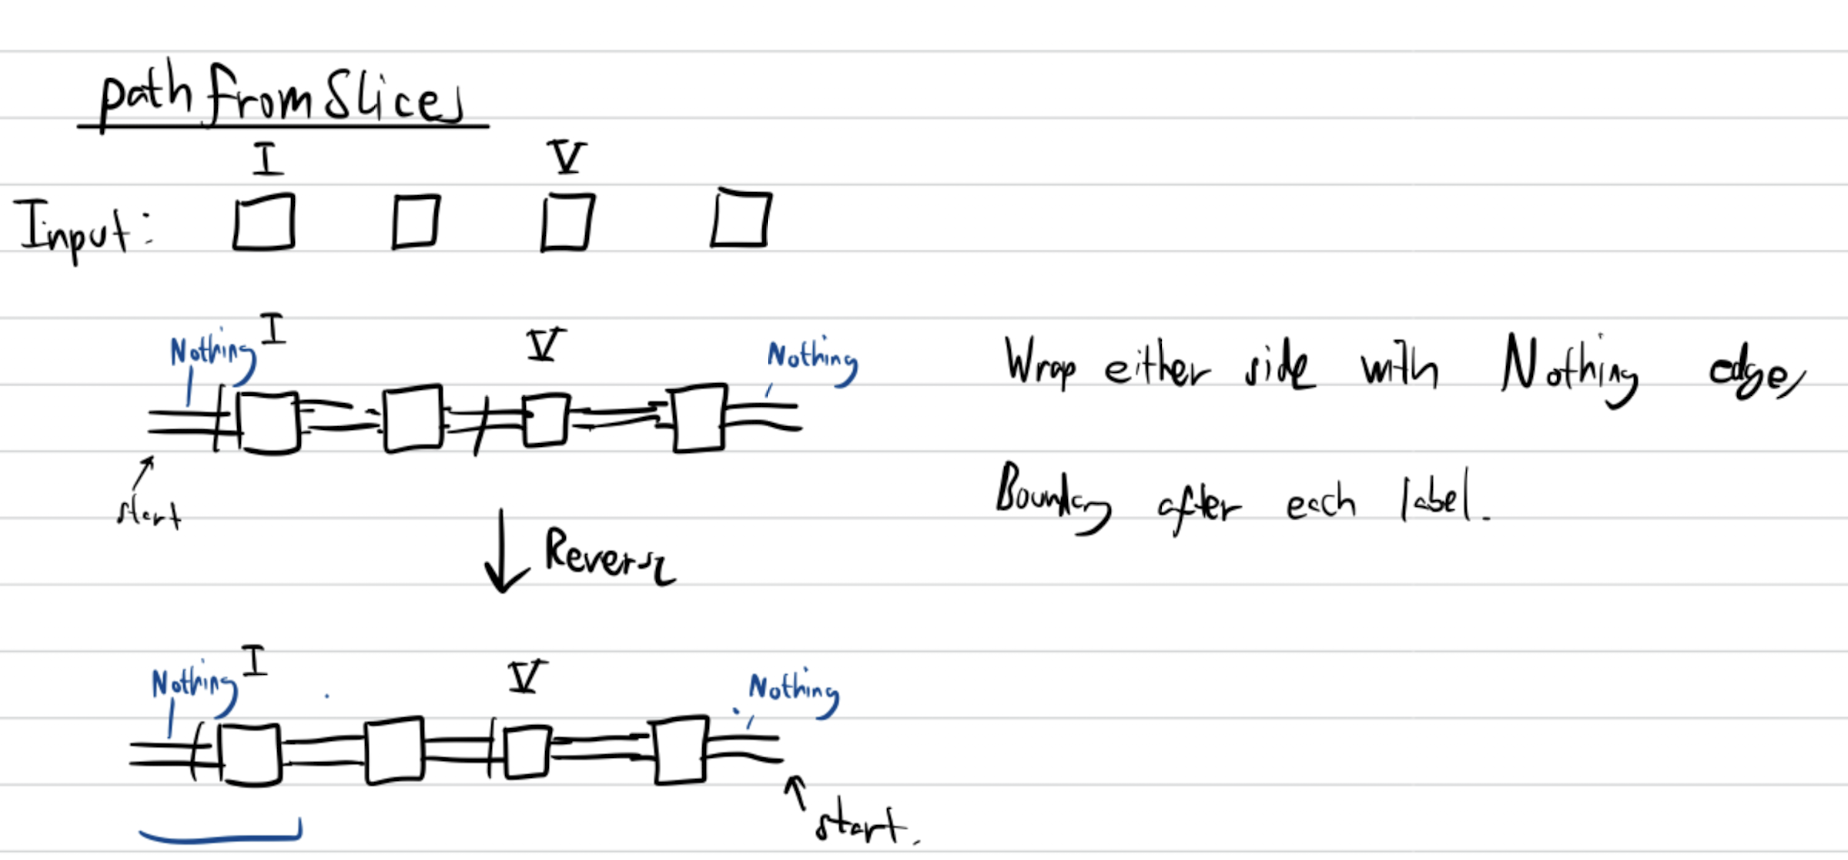
\includegraphics[width=\textwidth]{pathFromSlices}
  \caption{Path initiliasation}
  \label{fig:pathInit}
\end{figure}

\begin{definition}[Path]
A path is an alternating sequence of an two types of elements, in our case transitions and slices. Definition: Haskell code block or mathematical definition?
\end{definition}

Our goal is to reduce the piece into a partial redution by appluying operations until we have one slice per segment. Diagram of this state. This means we have one group of notes per segment, and this group of notes should represent the harmony of the segment.

We parse by applying the inverse of the generative operations, right to left. Unsplit, Unspread, Unfreeze.
\par


\begin{figure}[h]
  \centering
  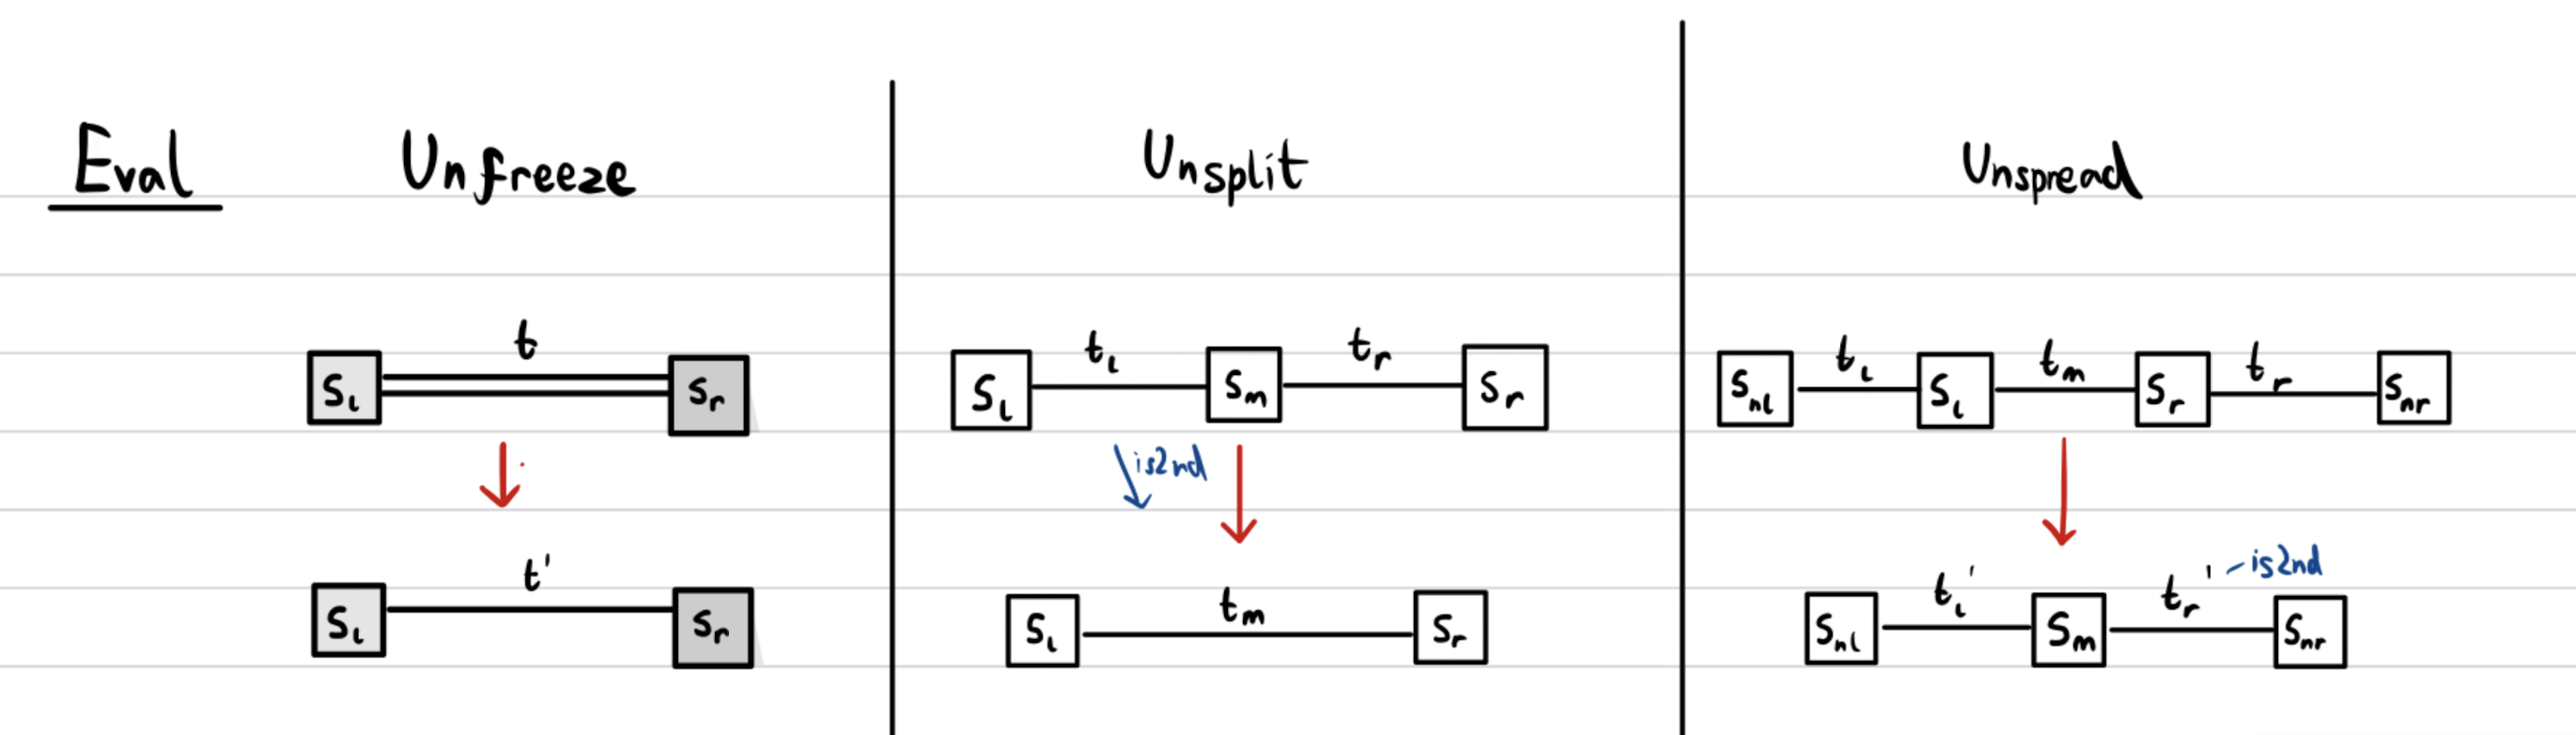
\includegraphics[width=\textwidth]{parseops}
  \caption{Parse operations}
  \label{fig:parseops}
\end{figure}

\FloatBarrier
\subsubsection{State Space}

This is how we define the search. We start at the right, the end of the piece. We have a pointer to the current node, and all preceeding slices are open and subsequent slices are frozen. Open Slices can be reduced, but only to the point that there is one slice in a segment. We keep track of the operations performed as it (1). allows us to the draw out the derivation for the partial reduction at the end, and (2). it is used later for calculate a cost for each operation for the heuristic search.




% \begin{figure}[h]
%   \centering
%   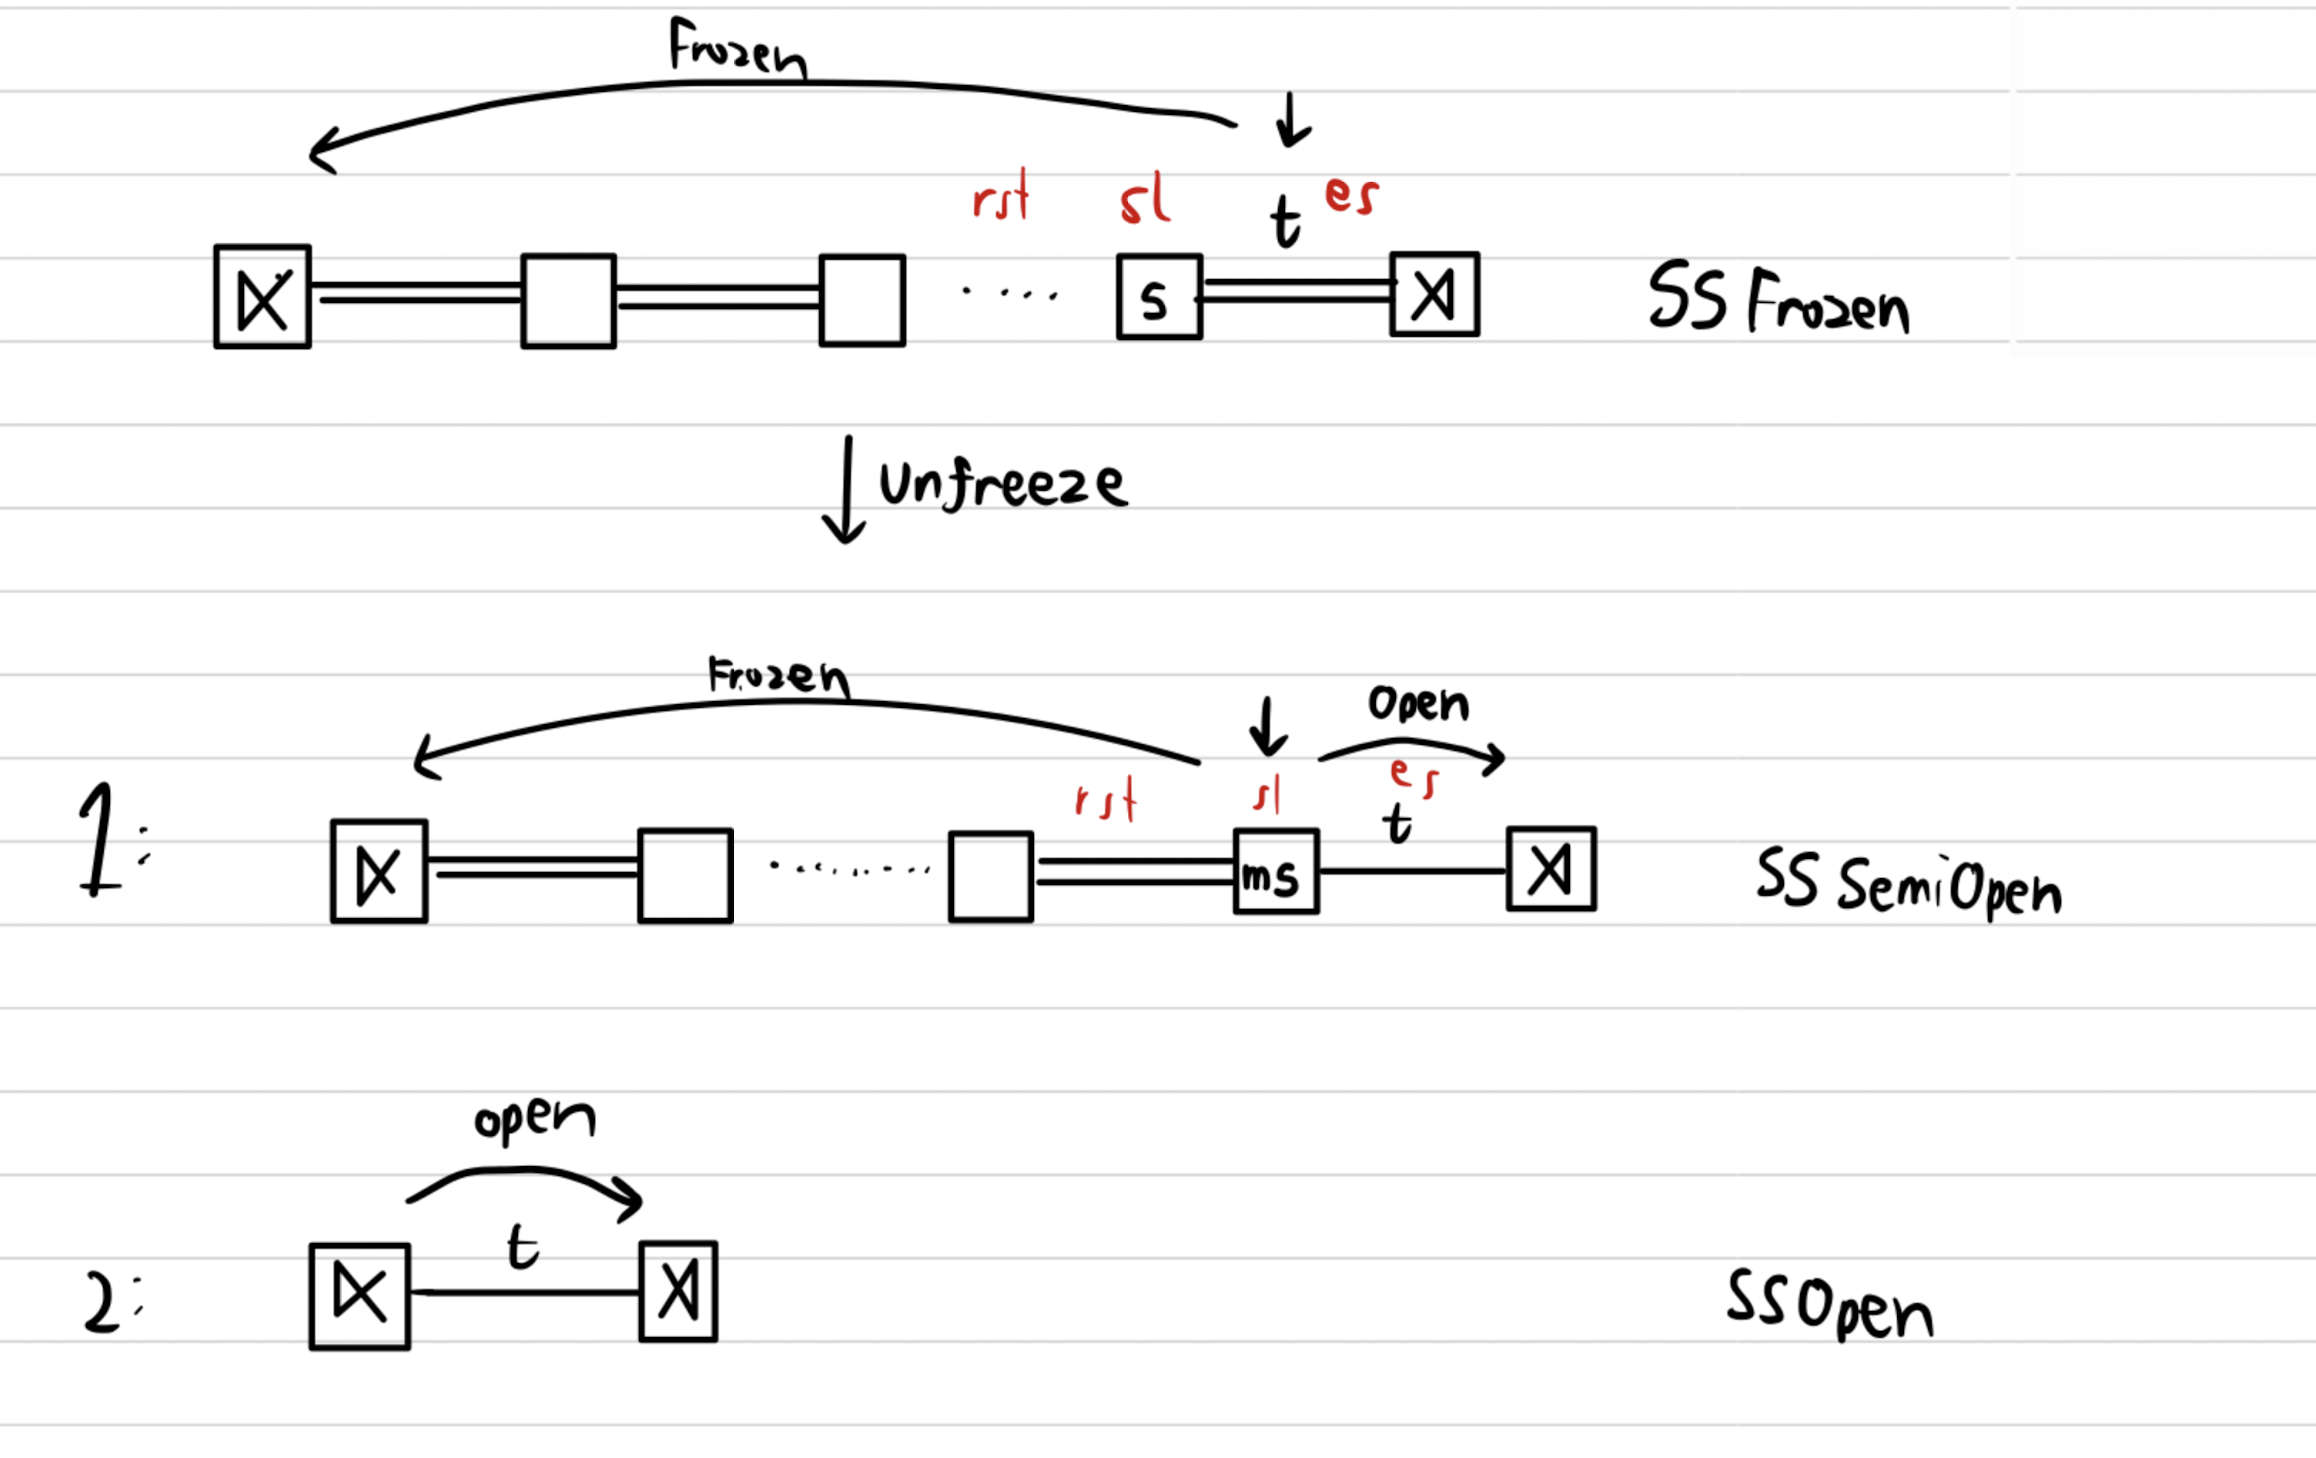
\includegraphics[width=\textwidth]{parsestates}
%   \caption{Parse operations}
%   \label{fig:parseops}
% \end{figure}

\begin{figure}[h]
  \centering
  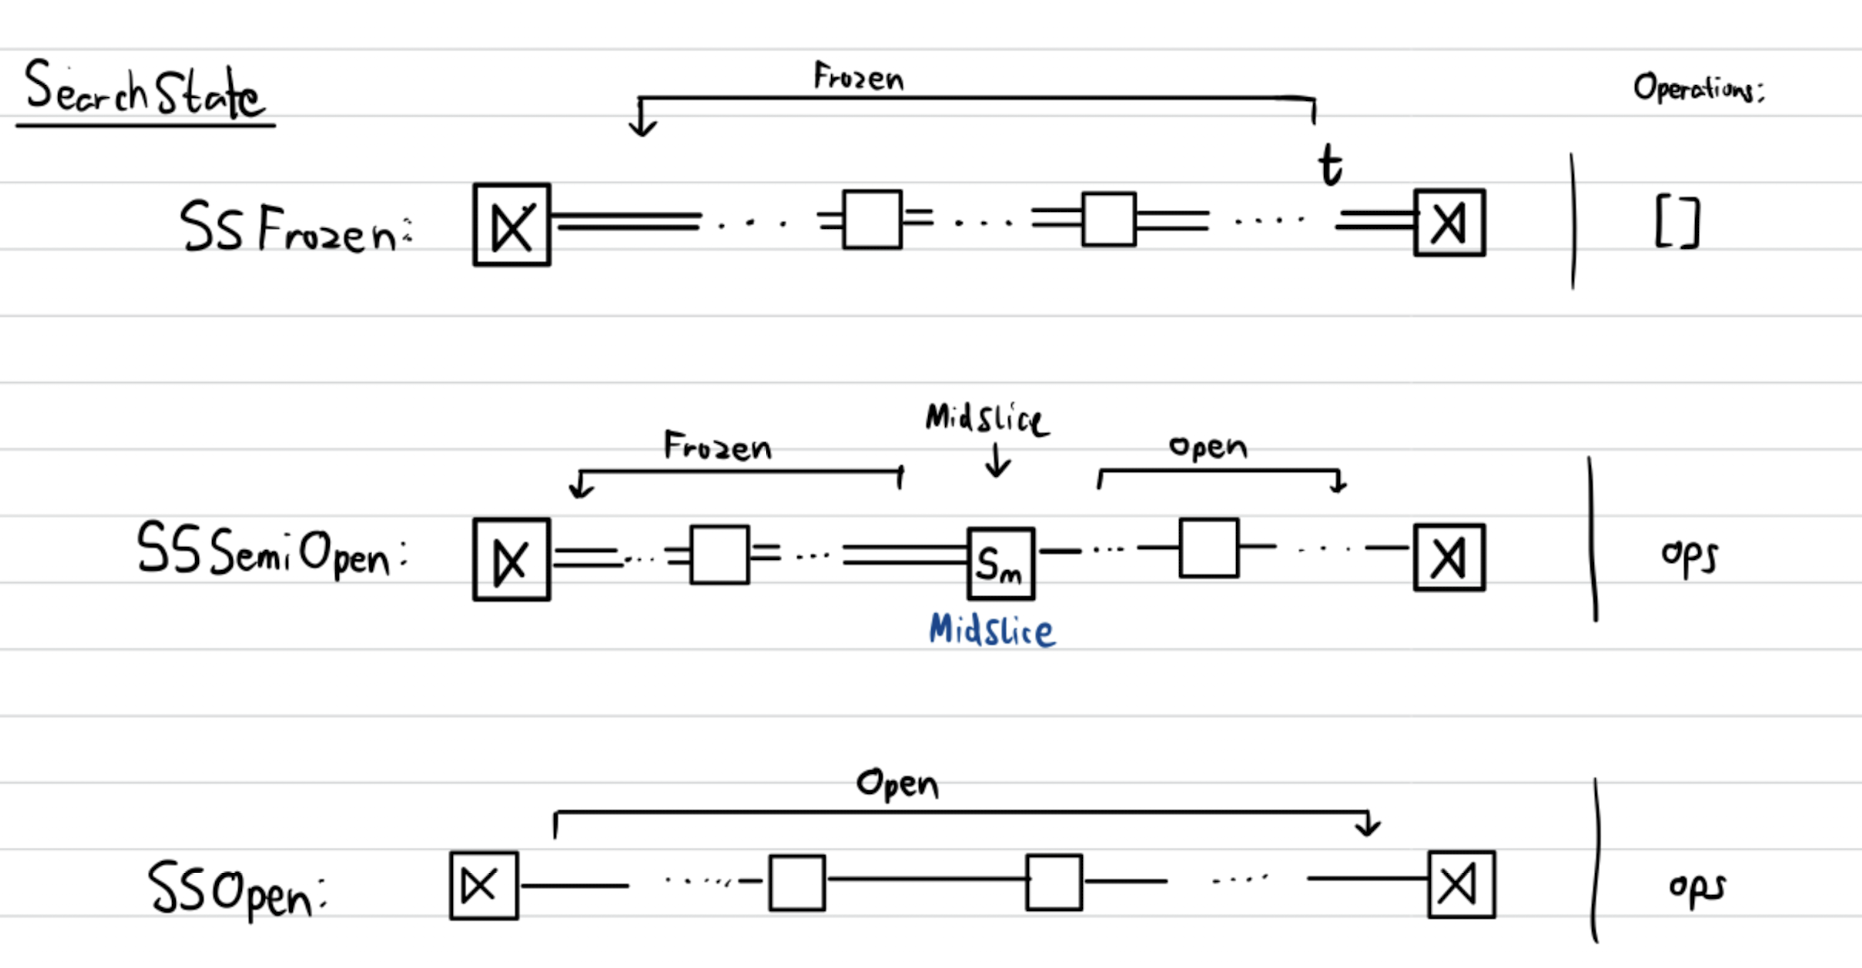
\includegraphics[width=\textwidth]{searchstate}
  \caption{Search state}
  \label{fig:searchstate}
\end{figure}
\par
\par

\FloatBarrier
\subsubsection{Enumerating State transitions}

\begin{figure}[h]
  \centering
  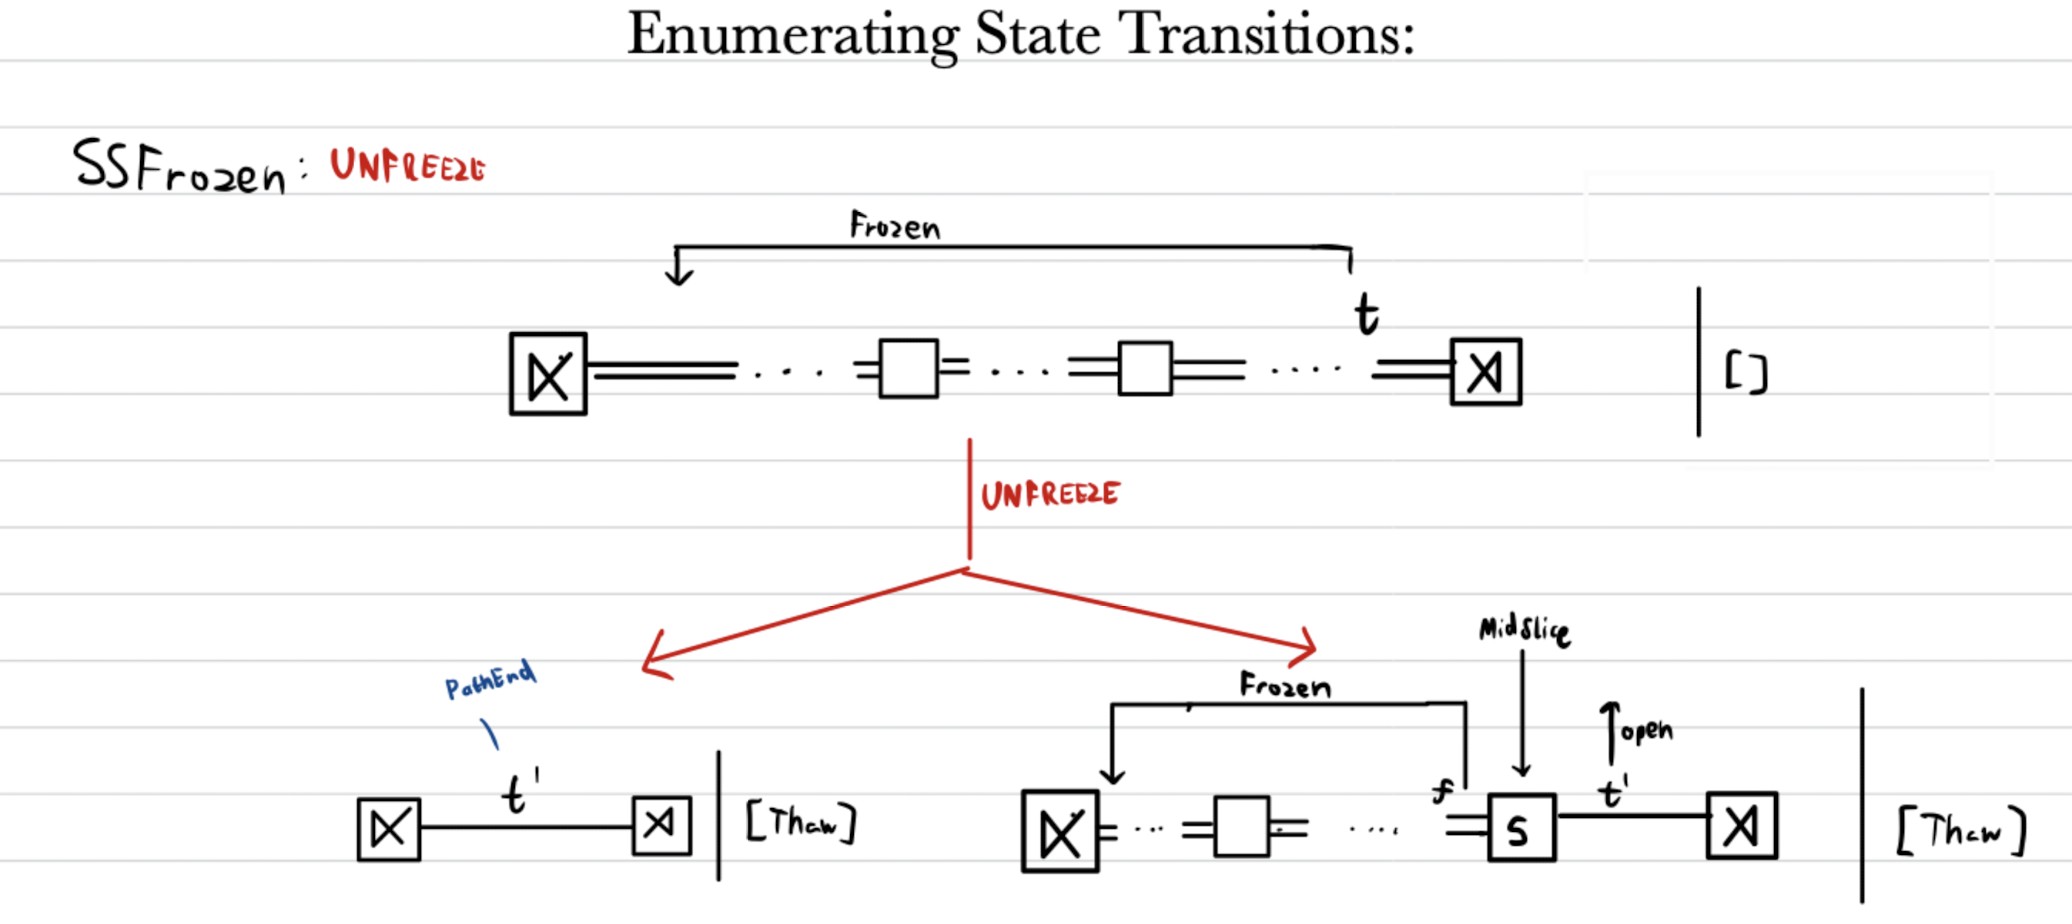
\includegraphics[width=0.7\textwidth]{frozenenum}
  \caption{Unfreeze operation}
  \label{fig:frozenenum}
\end{figure}


\begin{figure}[h]
  \centering
  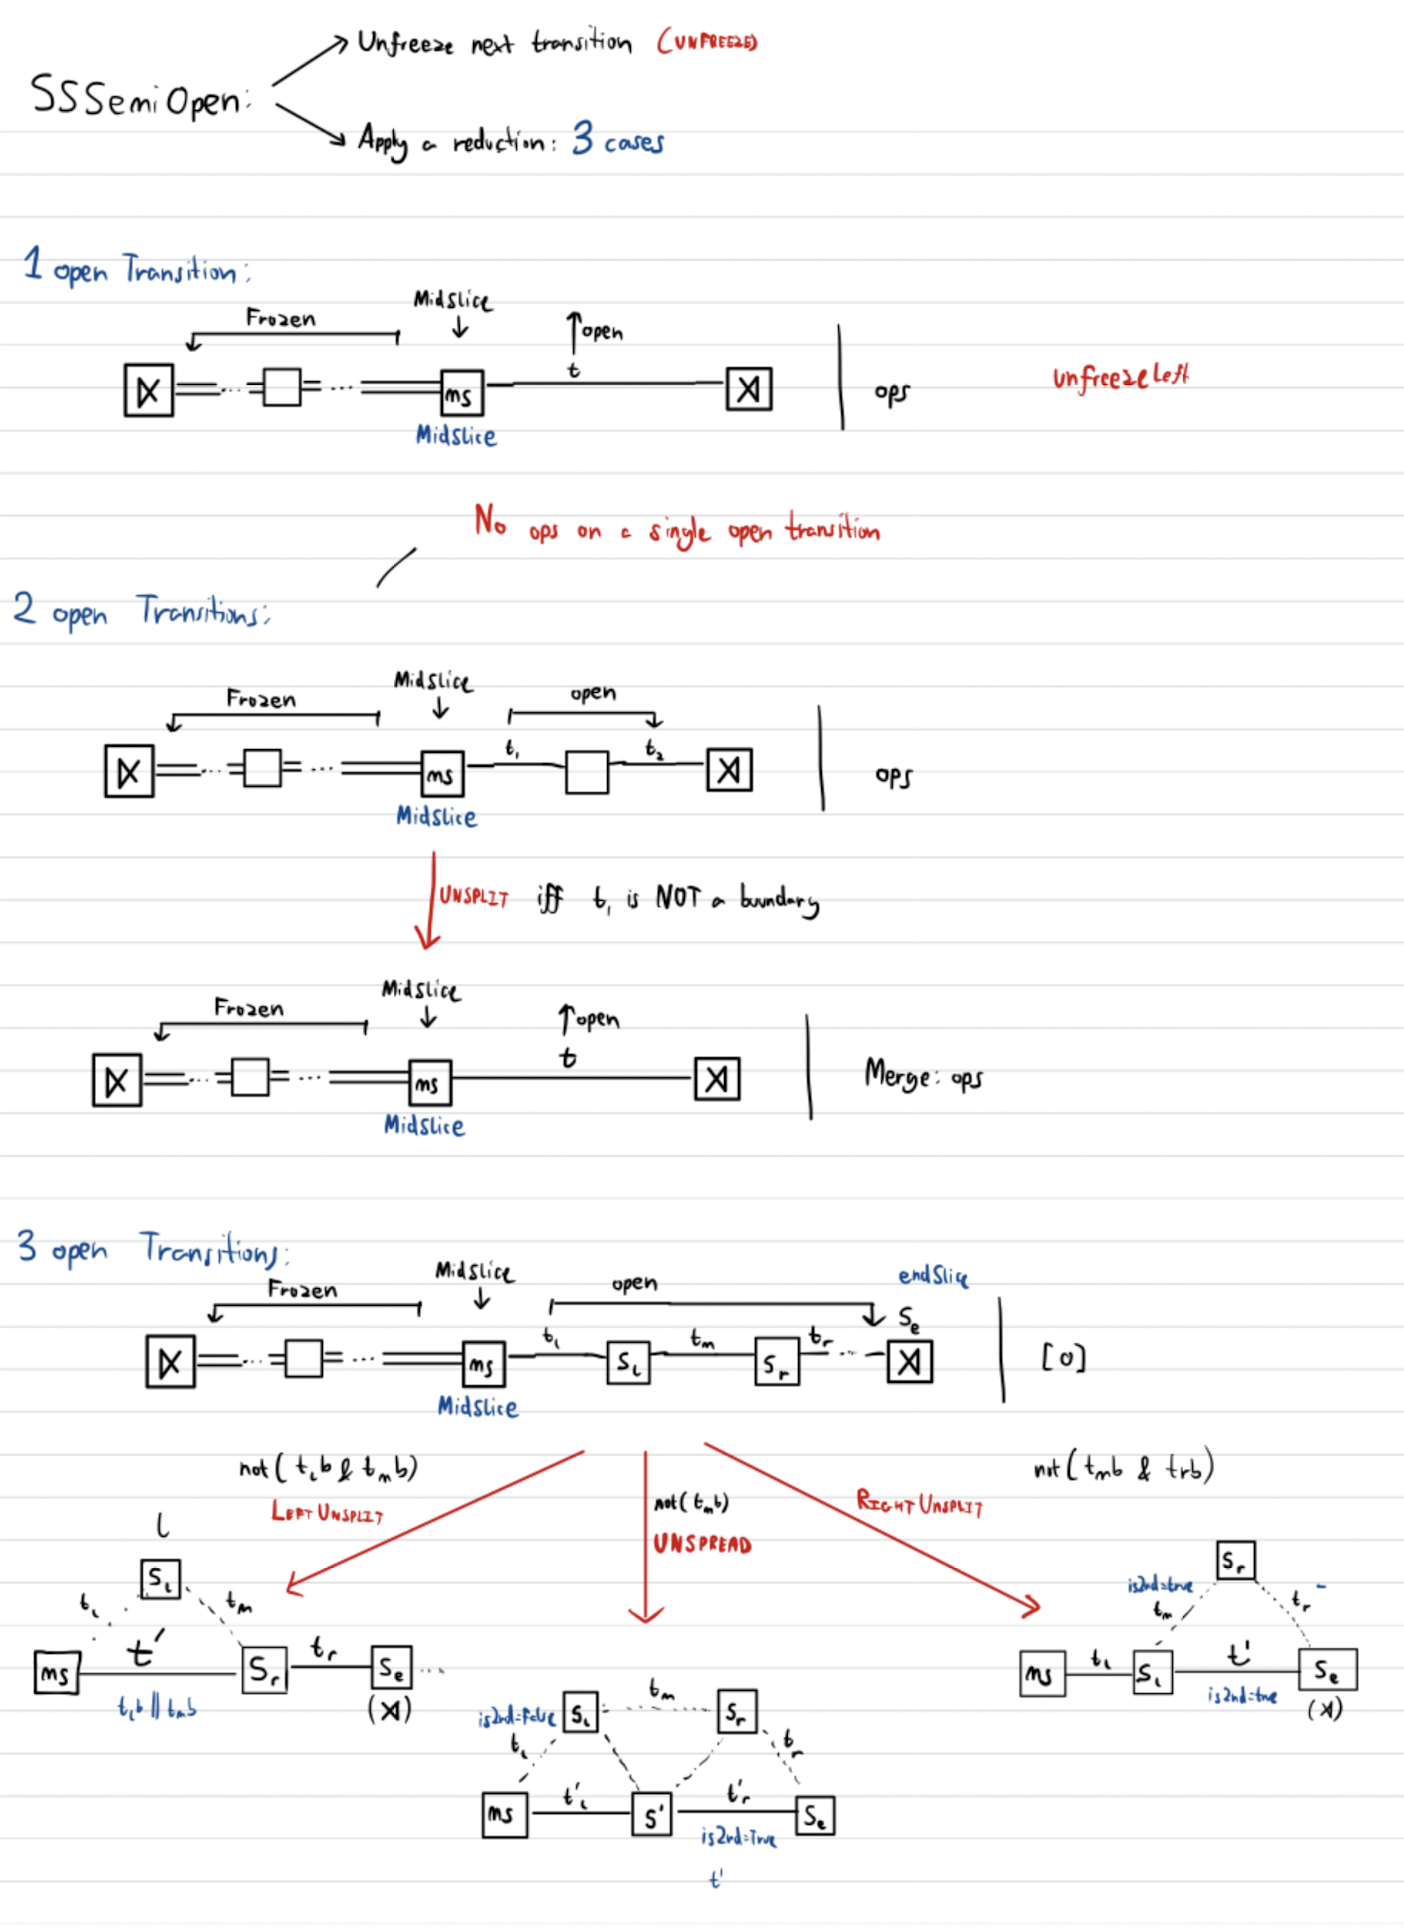
\includegraphics[width=0.7\textwidth]{sssemiopenenum}
  \caption{Enumeration of operations mid parse. Maybe for appendix? This could be much more concise.}
  \label{fig:sssemiopenenum}
\end{figure}

\begin{figure}[h]
  \centering
  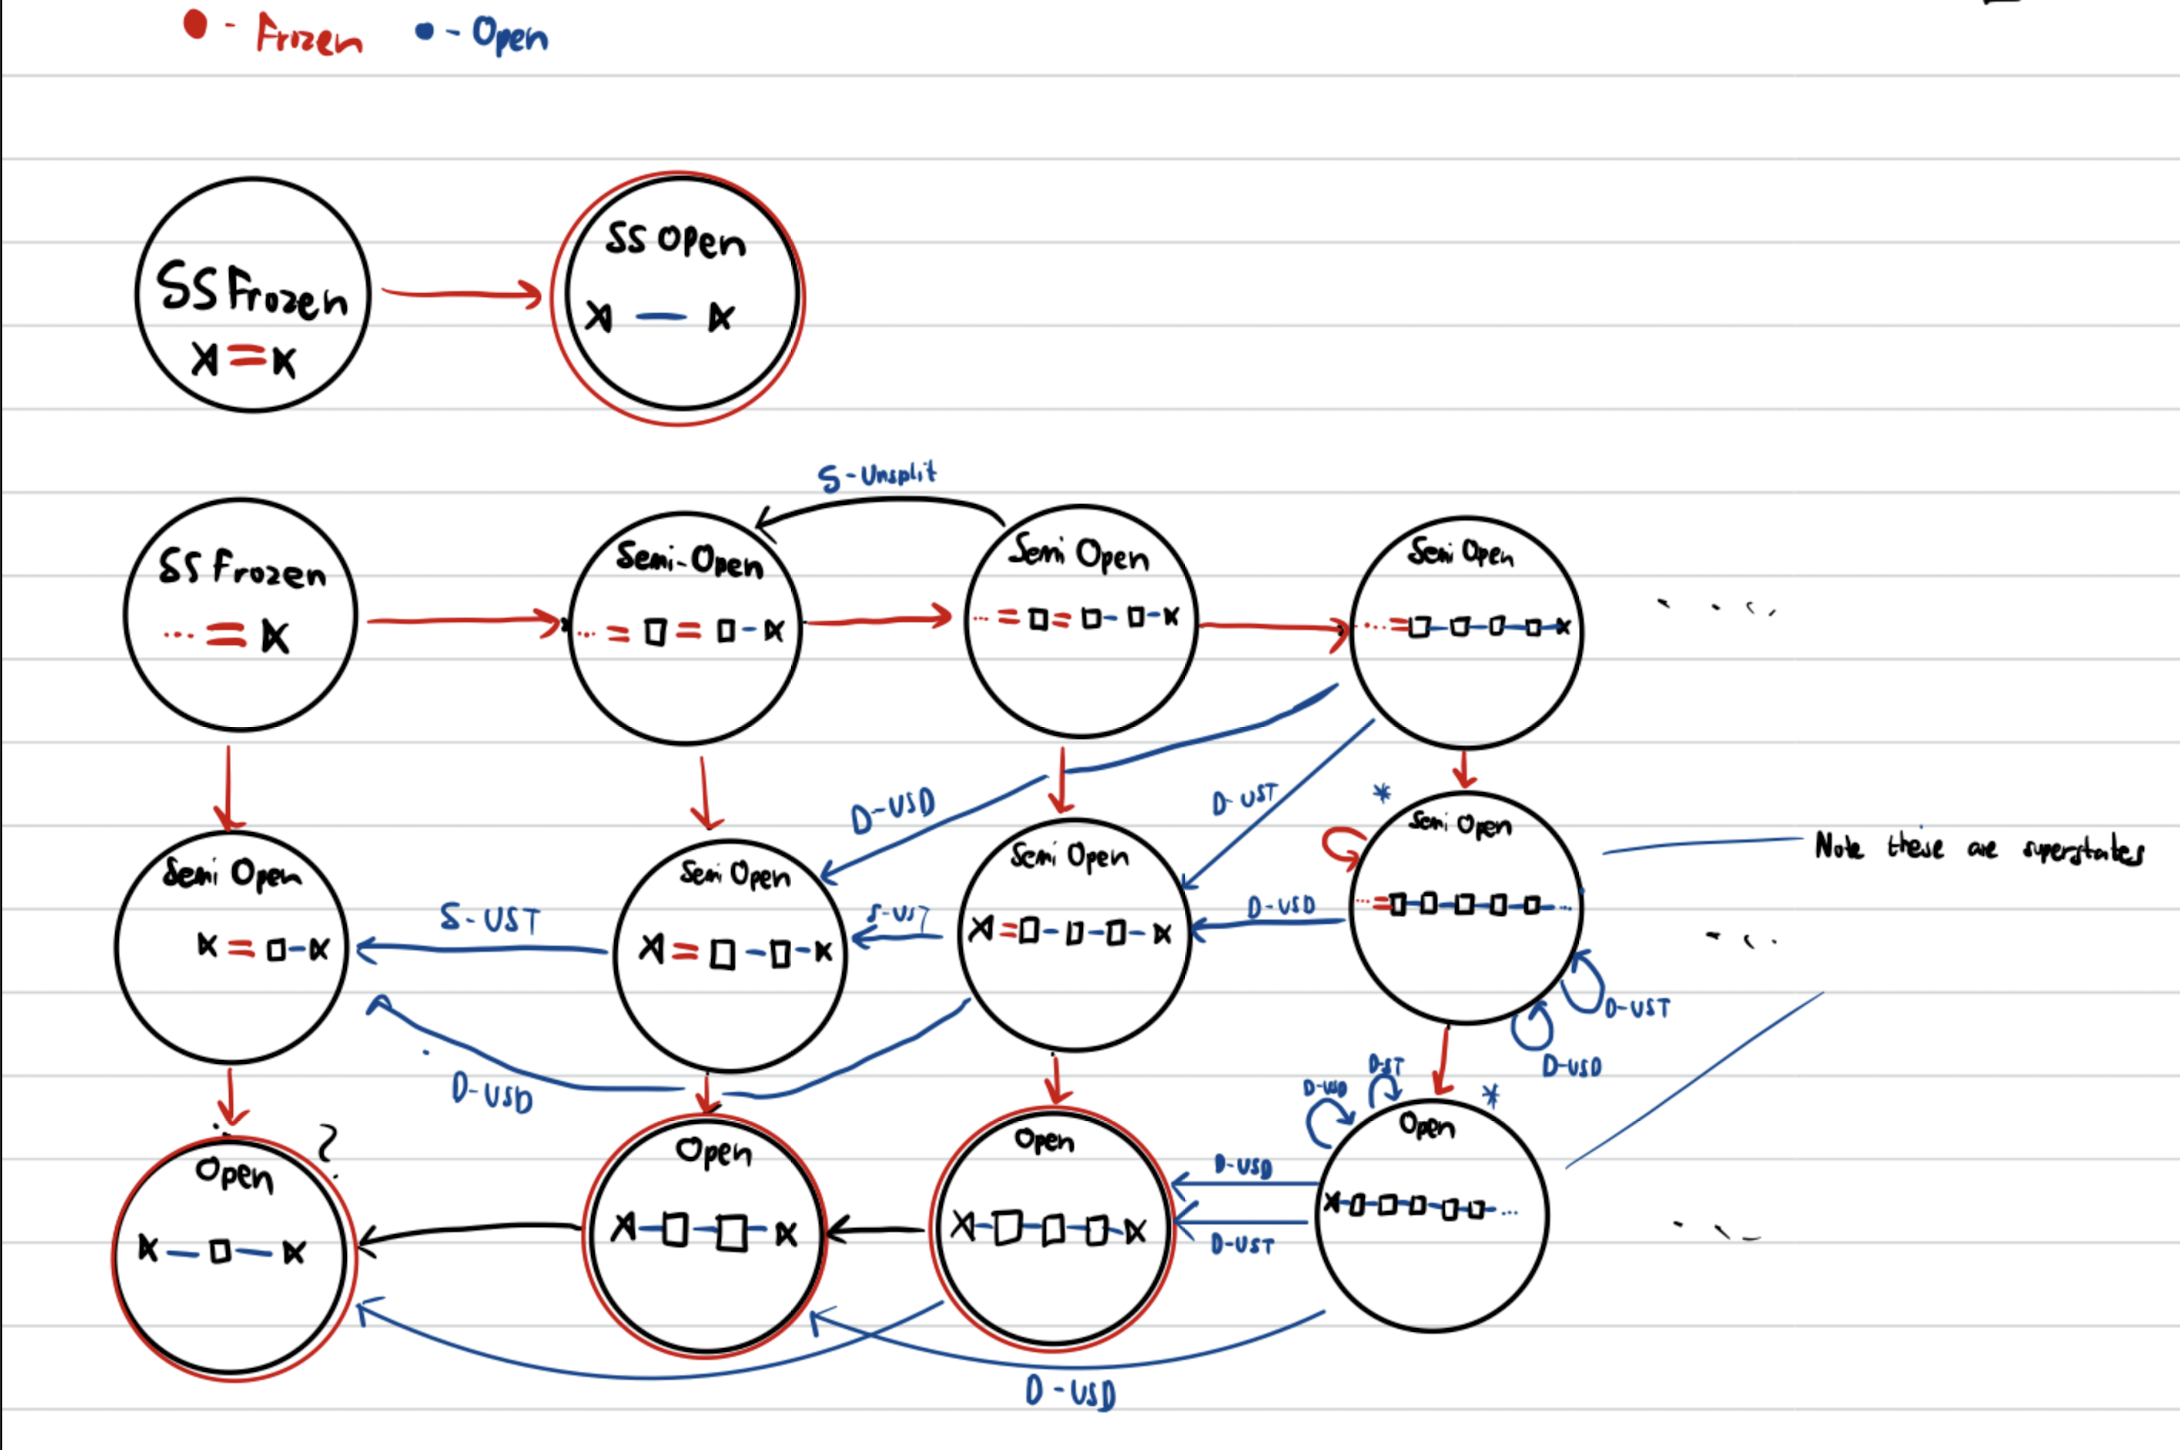
\includegraphics[width=\textwidth]{statetransitions}
  \caption{State Transition diagram}
  \label{fig:statetrans}
\end{figure}
\FloatBarrier

In the state transition diagram (Figure \ref{fig:statetrans}), we see all the possible parse states (Is this actually useful? Maybe for appendix). This was useful for me as it helps to conceptualise how the full parse actually works. The dimensions of this digramm of the search state depends on the length of the piece, and the size of each segment. We can see that there is a process of moving to the right to unfreeze transitions, and moving towards the left during reduction operations. Perhaps some simplification of the diagram would be useful. This transition diagram does not consider segment boundaries.

sdfsdfs

sdf

\FloatBarrier
\subsubsection{Boundary handling}

It is important thhat we don't reduce to an empty segment, because that would mean we've lost all information about the segment, and would not be able to make a harmonic inference. In order to prohibit this, we add additional constraints to the parse operations for each opertation based on the boolean boundary value of all involved transitions.
\par
We use karnaugh maps to determine the boolean expression for these constraints.

\begin{figure}[h]
  \centering
  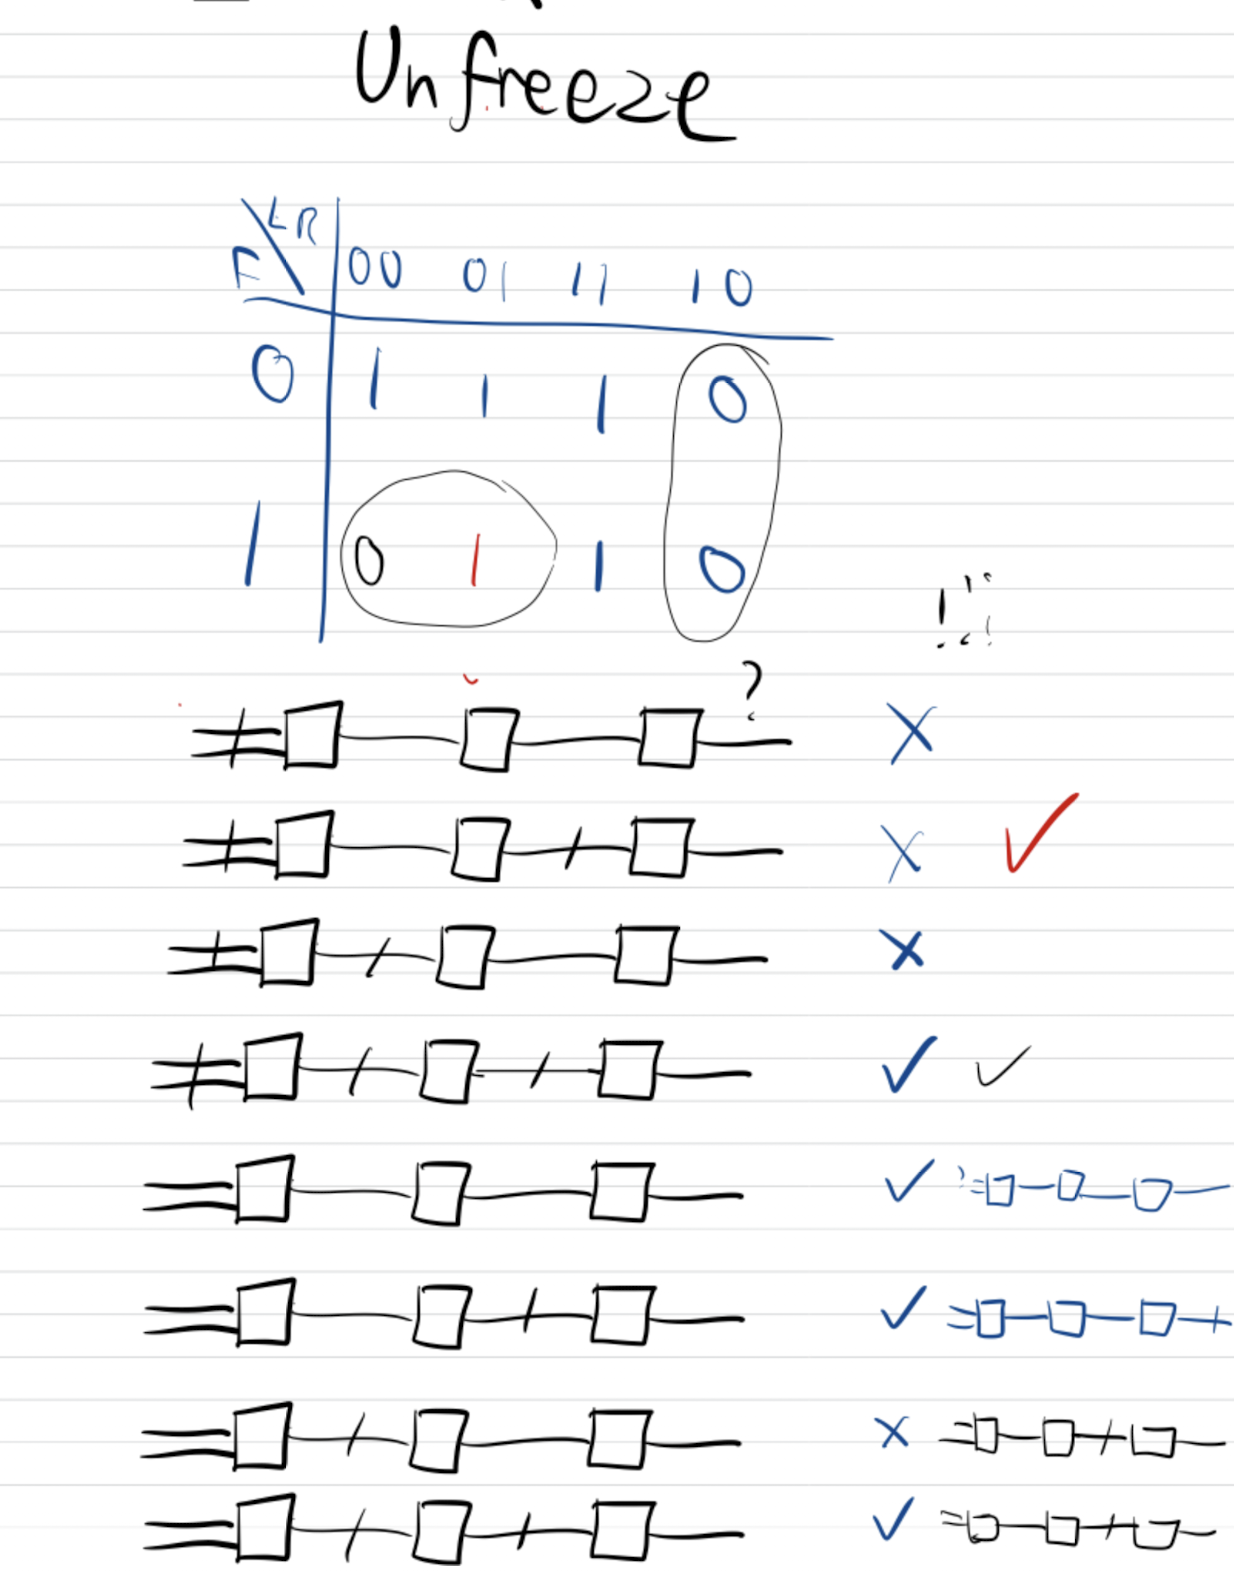
\includegraphics[width=0.7\textwidth]{karnaughunfreeze}
  \caption{Determine boolean boundary expressions for the freeze operations}
  \label{fig:karnaugh}
\end{figure}

\par 
Could show other maps in the appendix.


\FloatBarrier
\subsection{Evaluation Module}
We need to know exactly what we are trying to achieve before we can understand the baseline and extention implementations.

\FloatBarrier
\subsubsection{Probabilistic Model of Harmony}
When evaluating using the protovoice model: we assume that we result in only chord tones for each segment. Thus we can use the chord tone probabilities to evaluate the prediction. 
\par
When just using a random sample, we have to assume that there is a mixture model of chord tones and ornaments. We can use the learnt parameters to determine the distribution.
\par
These two measures of likelihoods are comparable as they are drawn from the same distributions.
\par
We also need to infer chord labels. We can simply choose the chord that is most likely according to our model.
\par 
This gives us two key metrics, likelihood and accuracy.
\par
Could also use a more sophisticated notion of accuracy, using a chord similarity function \cite{humphreyFourTimelyInsights2015}. The {\texttt {mir\_eval}} package provides a plethora of metrics to compare chord label predictions \cite{raffelMirEvalTransparent2014}. 

\section{Baseline implementation}


\subsection{Random Sample Parser}
As a crude baseline we develop two algorithms based on randomly sampling notes for each segment to infer the chord label. 
\par
The pure random sample algorithm simply samples random notes for each segment, and uses those to guess the chord label. This doesn't even consider the notes of the piece, so it's really bad, but provides a useful reference.
\par 
The per segment sample algorithm samples notes from each segment. Could just sample a random number of notes from each segment, or just use all the notes in the segment to predict the most likely chord label. This is reminiscent of using a key-profile model \cite{temperleyBayesianApproachKeyFinding2002} to find local keys.

\FloatBarrier
\subsection{Random Choice Search}
Now we use our implementation of the protovoice parser, but just do a random walk in the tree of partial reductions. By comparing this against the random ample parser, we can get an idea of the utility of the model. We show that this works surprisingly well.

\FloatBarrier
\section{Extension Implementation}

\subsection{Heuristic Design}
Step 1: Design heuristic to be as accurate as possible. I.e the extreme is to consider every possible parse, but for a single piece there can be over $10^{10^{10^{10^{10^{10}}}}}$ different parses. We consider 1 step at a time at first - this still results in needing to choose an operation out of upwards of 30,000,000 options for just a single step.     
\par
First the full piece heuristic parse 
\par
Problem of very large slices.\\ 
Segment by segment heuristic parse - avoids the problem, but is slightly hacky. Can we incorprate our knowledge regarding the relative proportion of chord tones and ornaments. Should we allow duplicates of notes in slices? Perhaps we should favour spreads more. 
\par
Always consider a certain number of slices and spreads.
\par

\begin{figure}[h]
  \centering
  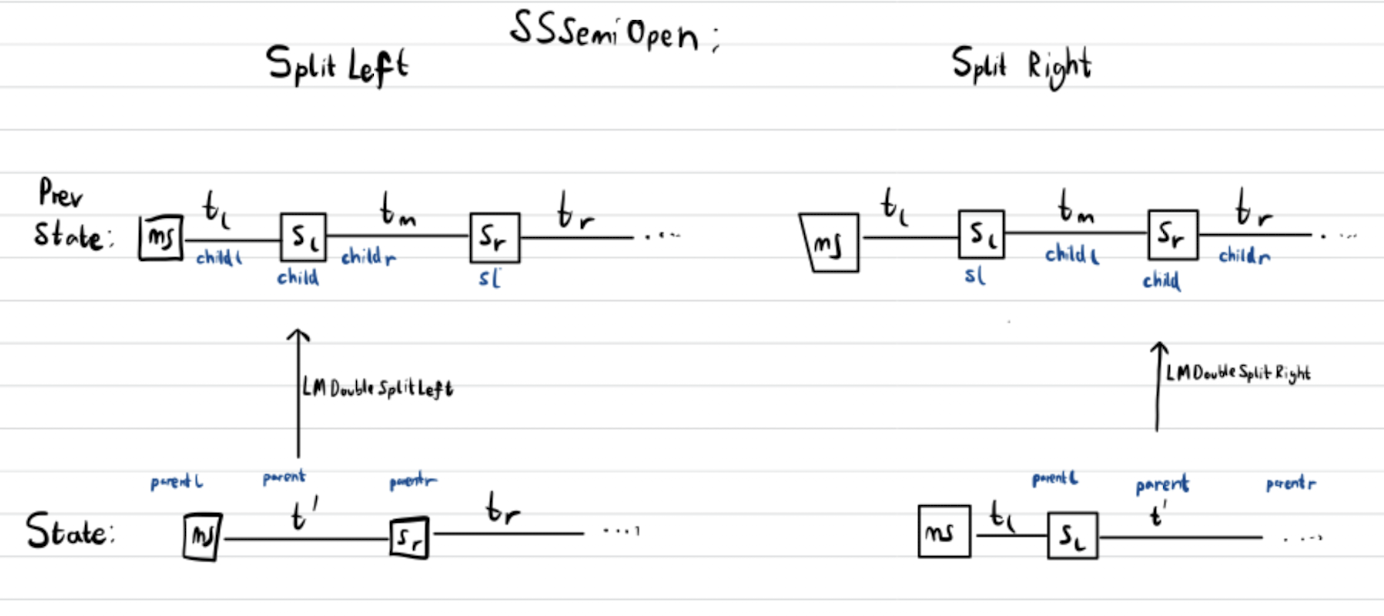
\includegraphics[width=0.7\textwidth]{splitsssemiopen}
  \caption{Split operation}
  \label{fig:splitoperation}
\end{figure}

\FloatBarrier
\subsubsection{Scoring Unsplit Operations}
Consider the Split rule : \[t \to t'_{l}~s'~t'_{r}\]
\par
During a split, each edge in the transition and each node in an adjacent slice can be elaborated by one or more inner operations.
These new edges can be discarded or kept to form the new edge of $t'_l$ and $t'_r$.
\par 
The notes in the child slice $s$ can either have edges connected to the left neighboring slice or right neighbouring slice, or both. I.e for each note in the child slice, it can be a an ornmentation of a previous note, subsequent note, both, or repetition of prev note, subsequent note etc. So we consider the chord tone profiles of the involved slices. 

We first guess the chord type each parent slice. 
\[\theta_l = \mathop{argmax}_{c \in C} P(s_l|c) ~~,~~ \theta_r = \mathop{argmax}_{c \in C} P(s_r|c) '\]

We now consider each edge individually, considering their likelihoods based on the proabilistic model of harmony along with theoretical assumptions. 

\paragraph{Single Sided Operations} 
\begin{itemize}
  \item Right Neighbour (Left Neighbour anagolously)
    \[ x \implies x \to n~~, x,n \in P \]
    \[x \sim \text{Categorical}(\sigma_{ct}^{\theta_l})\]
    \[n \sim \text{Categorical}(\sigma_{or}^{\theta_r})\]
    Find \[P(x,n~|~\theta_l)\]
  \item Right Repeat (Left Repeat anagolously)
    \[ x \implies x \to x~~, x \in P \]
    \[x \sim \text{Categorical}(\sigma_{ct}^{\theta_l})\]
    Find \[P(x~|~\theta_l)\]
\end{itemize}
\paragraph{Two Sided Operations} 
\begin{itemize}
  \item Root Note: This operation is only done once in the original model. In our case we do not need to consider due to segment boundaries.
  \item Full Repeat: 
    \[ x \implies x \to n~~, x,n \in P \]
    \[x \sim \text{Categorical}(\sigma_{ct}^{\theta_l})\]
    \[n \sim \text{Categorical}(\sigma_{or}^{\theta_r})\]
    Find \[P(x,n~|~\theta_l)\]
  \item Left Repeat of Right: 
    \[ x \to y \implies x \to y' \to y \]
    \[y \sim \text{Categorical}(\sigma_{ct}^{\theta_l})\]
    Find \[P(y~|~\theta_l)\]
  \item Full Neighbour:
    \[ x_1 \to x_2 \implies x_1 \to n \to x_2, x \in P \]
    % \[x \sim \text{Categorical}(\sigma_{ct}^{\theta_l})\]
    Find \[P(|~\theta_l,\theta_r)\]
\end{itemize}

\FloatBarrier
\subsubsection{Scoring Unspread Operations}

Consider the Spread rule : \[t_l s_r \to t'_l s_l t'_m s_r t'_r\]
We make the assumption that $s$, $s_l$, \& $s_r$ are all realisations of the same chord. This lines up with the music theorretical basis for this operation in the model(justify).
\par 
Thus we find the most likely chord (optional extension: marginalise over all chords)
\[\theta = \mathop{argmax}_{c \in C} P (s|c)\]
\par 
When then measure the extent to which the parent slics match this chord.

\[p(s_l, s_r| \theta)\]

We can calculate $p(s_l|\theta)$ and $p(s_r|\theta)$ using the multinomial distribution probability density function as described in the preparation chapter.

\FloatBarrier
\subsubsection{Scoring Unfreeze Operations}
We assign 0 cost to unfreeze operations. This means we need to be careful about ensure that we don't just unfreeze the entire piece immediately. Careful construction of the search algorithm can ensure this. More later.

\FloatBarrier
\subsubsection{Full state evalutation}
We need to combine all of these in a fair way. Also the distinction between splits and spreads need to be considred, as they are different operations, the calculations of likelihood may cause an imbalance. 

\FloatBarrier
\subsection{Heuristic Search}
Step 2: Relax the heuristic search in order to reduce runtime/ lower complexity.
\par 
In the case that there are 85,000,000 options, perhaps we should sample the options rather than evaluating all of them. 
\par 
This version of heuristic search should be able to parse full pieces (hopefully), so can be used to compare with the baselines on an entire corpus.



\section{Testing}
Show unit tests, and examples of the test/development cycle for the heuristic search development

%%%%%%%%%%%%%%%%%%%%%%%%%%%%%%%%%%%%%%%%%%%%%%%%%%%%%%%%%%%%%%%%%%%%%
% Evaluation
%%%%%%%%%%%%%%%%%%%%%%%%%%%%%%%%%%%%%%%%%%%%%%%%%%%%%%%%%%%%%%%%%%%%%

\chapter{Evaluation}
\textit{In this chapter, I provide qualitative and quantitative evaluations of the work completed. I then provide and interpret evidence to show that the success criteria were met.}

\textit{The main questions to answer are as follows:}
\begin{itemize}
  \item \textit{Can the proto-voice model be used to accurately infer chord labels?}
  \item \textit{Can the proto-voice model be used to practically infer chord labels?}
  \item \textit{How well my heuristic search algorithms infer chord labels?}
\end{itemize}

\section{Accuracy}
Things to note
\begin{itemize}
  \item The fact that segmentation is known ahead of time provides a great deal of information \cite{gothamWhatIfWhen2021}
  \item So we can use comparisons between the random sample from each segment algorithm and the random parse algorithm to see if the use of the grammar provides an advantage over just sampling the notes directly, without looking at relations between notes.
  \item Then we want a heuristic search algorithm that considers each option exhaustively and finds the best local option. This is too computationally expensive to be used for whole pieces. 
  \item Given there can be millions of possible next states in the search, we need to look at different strategies to avoid searching through them all. E.g just sample states. 
  \item Sensitivity Analysis for the heuristic search is useful for the evaluation. Explore how robust it is to handcrafted attacks/ different types of passages.
  \item Could evaluate by segments instead of pieces. 
\end{itemize}

\section{Performance}

\section{Heuristic Search (Extension)}

\section{Success Criteria}

\section{Limitations}


%%%%%%%%%%%%%%%%%%%%%%%%%%%%%%%%%%%%%%%%%%%%%%%%%%%%%%%%%%%%%%%%%%%%%
% Conclusions
%%%%%%%%%%%%%%%%%%%%%%%%%%%%%%%%%%%%%%%%%%%%%%%%%%%%%%%%%%%%%%%%%%%%%

\chapter{Conclusions}
\textit{In this chapter, I first discuss the success achieved by the project then offer a reflection on lessons learned. Finally, I consider the directions in which there is potential for future work.}
\section{Achievements}

\section{Lessons learned}

\section{Future Work}

\cite{finkensiep_modeling_2021}


%%%%%%%%%%%%%%%%%%%%%%%%%%%%%%%%%%%%%%%%%%%%%%%%%%%%%%%%%%%%%%%%%%%%%
% the bibliography
%%%%%%%%%%%%%%%%%%%%%%%%%%%%%%%%%%%%%%%%%%%%%%%%%%%%%%%%%%%%%%%%%%%%%
\addcontentsline{toc}{chapter}{Bibliography}
\nocite{*}
% \addbibresource{Disseration.bib}
\bibliography{Dissertation}


%%%%%%%%%%%%%%%%%%%%%%%%%%%%%%%%%%%%%%%%%%%%%%%%%%%%%%%%%%%%%%%%%%%%%
% the appendices
%%%%%%%%%%%%%%%%%%%%%%%%%%%%%%%%%%%%%%%%%%%%%%%%%%%%%%%%%%%%%%%%%%%%%

\appendix

\chapter{Additional Information}

% \section{metadata.tex}
% {\scriptsize\verbatiminput{metadata.tex}}
%
% \section{main.tex}
% {\scriptsize\verbatiminput{main.tex}}
%
% \section{proposal.tex}
% {\scriptsize\verbatiminput{proposal.tex}}
%
% \chapter{Makefile}
%
% \section{makefile}\label{makefile}
% {\scriptsize\verbatiminput{makefile.txt}}
%
% \section{refs.bib}
% {\scriptsize\verbatiminput{refs.bib}}


\chapter{Project Proposal}

% Note: this file can be compiled on its own, but is also included by
% diss.tex (using the docmute.sty package to ignore the preamble)
\documentclass[12pt,a4paper,twoside]{article}
\usepackage[pdfborder={0 0 0}]{hyperref}
\usepackage[margin=25mm]{geometry}
\usepackage{graphicx}
\usepackage{parskip}
\begin{document}

\begin{center}
\Large
Computer Science Tripos -- Part II -- Project Proposal\\[4mm]
\LARGE
How to write a dissertation in \LaTeX\\[4mm]

\large
M.~Richards, St John's College

Originator: Dr M.~Richards

14 October 2011
\end{center}

\vspace{5mm}

\textbf{Project Supervisor:} Dr M.~Richards

\textbf{Director of Studies:} Dr M.~Richards

\textbf{Project Overseers:} Dr F.~H.~King  \& Dr A.~W.~Moore

% Main document

\section*{Introduction}

\emph{The problem to be addressed.}

Many students write their CST dissertations in \LaTeX\ -- and spend a
fair amount of time learning just how to do that. The purpose of this
project is to write a demonstration dissertation that provides
a starting point to show how it is done.

This core proposal document will be augmented by a separately-printed
cover sheet at the front and a resource form at the end. Additional
sheets for risk assessment and human resources may also need to be
included.

This document will elaborate much of the material that is summarised on
the additional sheets.

\section*{Starting point}

\emph{Describe existing state of the art, previous work in this area,
  libraries and databases to be used. Describe the state of any
  existing codebase that is to be built on.}

I am already able to write prose using the English language. I have an
online dictionary, etc.

\section*{Resources required}

\emph{A note of the resources required and confirmation of access.}

For this project I shall mainly use my own quad-core computer that
runs Fedora Linux. Backup will be to github and/or to an SVN
repository on an external hard disk that is dumped to writable CD/DVD
media. I have another similar computer to hand should my main machine
suddenly fail. I require no other special resources.

\section*{Work to be done}

\emph{Describe the technical work.}

The project breaks down into the following sub-projects:

\begin{enumerate}

\item The construction of a skeleton dissertation with the required
  structure. This involves writing the Makefile and making dummy
  files for the title page, the proforma, chapters 1 to 5, the
  appendices and the proposal.

\item Filling in the details required in the cover page and proforma.

\item Writing the contents of chapters 1 to 5, including examples of
  common \LaTeX\ constructs.

\item Adding a example of how to use floating figures and ``encapsulated
  PostScript'' or PDF diagrams.

\end{enumerate}

\section*{Success citeria}

\emph{Describe what you expect to be able to demonstrate at the
end of the project and how you are going to evaluate your achievement.}

The project will be a success if I have a completed dissertation with
the correct chapter titles and I have achieved my other success
criteria, which are to blah \ldots


\section*{Possible extensions}

{\em Potential further envisaged evaluation metrics or extensions.}

If I achieve my main result early I shall try the following
alternative experiment or method of evaluation \ldots


\section*{Timetable}

\emph{A workplan of perhaps ten or so two-week work-packages,
as well as milestones to be achieved along the way. Provide a
target date for each milestone.}

Planned starting date is 16/10/2011.

\begin{enumerate}

\item \textbf{Michaelmas weeks 2--4} Learn to use X. Read book Y. Read papers Z.

\item \textbf{Michaelmas weeks 5--6} Do preliminary test of Q.

\item \textbf{Michaelmas weeks 7--8} Start implementation of main task A.

\item \textbf{Michaelmas vacation} Finish A and start main task B.

\item \textbf{Lent weeks 0--2} Write progress report. Generate corpus of
  test examples. Finish task B.

\item \textbf{Lent weeks 3--5} Run main experiments and achieve working project.

\item \textbf{Lent weeks 6--8} Second main deliverable here.

\item \textbf{Easter vacation:} Extensions and writing dissertation main
  chapters.

\item \textbf{Easter term 0--2:}  Further evaluation and complete dissertation.

\item \textbf{Easter term 3:} Proof reading and then an early submission
  so as to concentrate on examination revision.

\end{enumerate}

\end{document}

\end{document}
